The aim of this paper is to evaluate for the purpose of determining travel patterns of Argentinian residents.
The exploratory data analysis aimed to describe the tweets based on whether they had a location mention, a geotag or both.

%The questions we aimed to answer with the exploratory data analysis
%\begin{enumerate}
%    \item What are the mentioned locations in tweets?
%    \item What are the geotagged locations in tweets?
%    \item How often are mentioned locations the same as geotagged locations?
%\end{enumerate}

Geotagged tweets were defined as those that contain a non-null Place and Coordinate objects. Mentioned tweets were defined as those that contained an NER tag {\fontfamily{qcr}\selectfont LOC} in the tweet content. Geoparsed tweets were mentioned tweets that have been mapped to coordinates by Google Geolocator API.

\section{Composition of the Tweet Collection}

There were a total of 182,571,272 tweets from 89,369 users whose tweets were collected and processed.
56435136 (30.91\%)  of those tweets were geotagged,  7,269,062 (3.98\%) had a location mention,  3,186,664 (1.75\%) had a geoparsed location. There were 3,015,837  tweets that had both a geotag and a location mention (corresponding to 82342  users); of which  1,722,811  tweets have a geotag and geoparsed location (corresponding to 72898  users). 

Over the relevant time period, Table \ref{fig:results-venn-diagram} shows the summary statistics of tweets per user.

Figure \ref{fig:results-venn-diagram} shows the overlap between geotagged, mentioned, and geoparsed tweets among the total collected tweets.
Users may have had more than one mentioned location per tweet, and had varying patterns of geotagging and mentioning.
A small subset of users were found to have very high rates of geotagging/mentioning and upon closer inspection, appeared to be event promoters or similar accounts.

\begin{figure}[H]
    \centering
    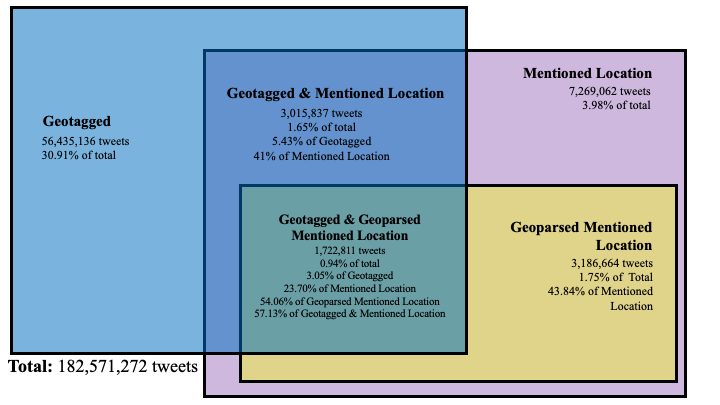
\includegraphics[width=1\textwidth]{images/Results-Venn-Diagram.png}
    
    \caption{Summary of Collected Tweets}
    \label{fig:results-venn-diagram}
\end{figure}

\begin{table}[htbp]
    \centering
    \begin{tabular}{|c|c|c|c|c|}
    \hline
    \textbf{Metric} & \textbf{Total} & \textbf{Geotagged} & \textbf{Mentioned} & \textbf{Geoparsed}\\
    \hline
    Mean &  2042.89  &  631.77  &  83.00  &  38.25 \\
    
    Median &  1164.0  &  286.0  &  34.0  &  13.0 \\
    
    Max &  155484  &  155464  &  79546  &  74832 \\
    
    Min &  1  &  1  &  1  &  1 \\ 
    
    Std &  2822.51  &  1208.67  &  397.92  &  329.78 \\
    \hline
    \end{tabular}
    \caption{Summary of Number of Tweets per User}
    \label{tab:summary-users}
\end{table}

%\begin{figure}[H]
%    \centering
%    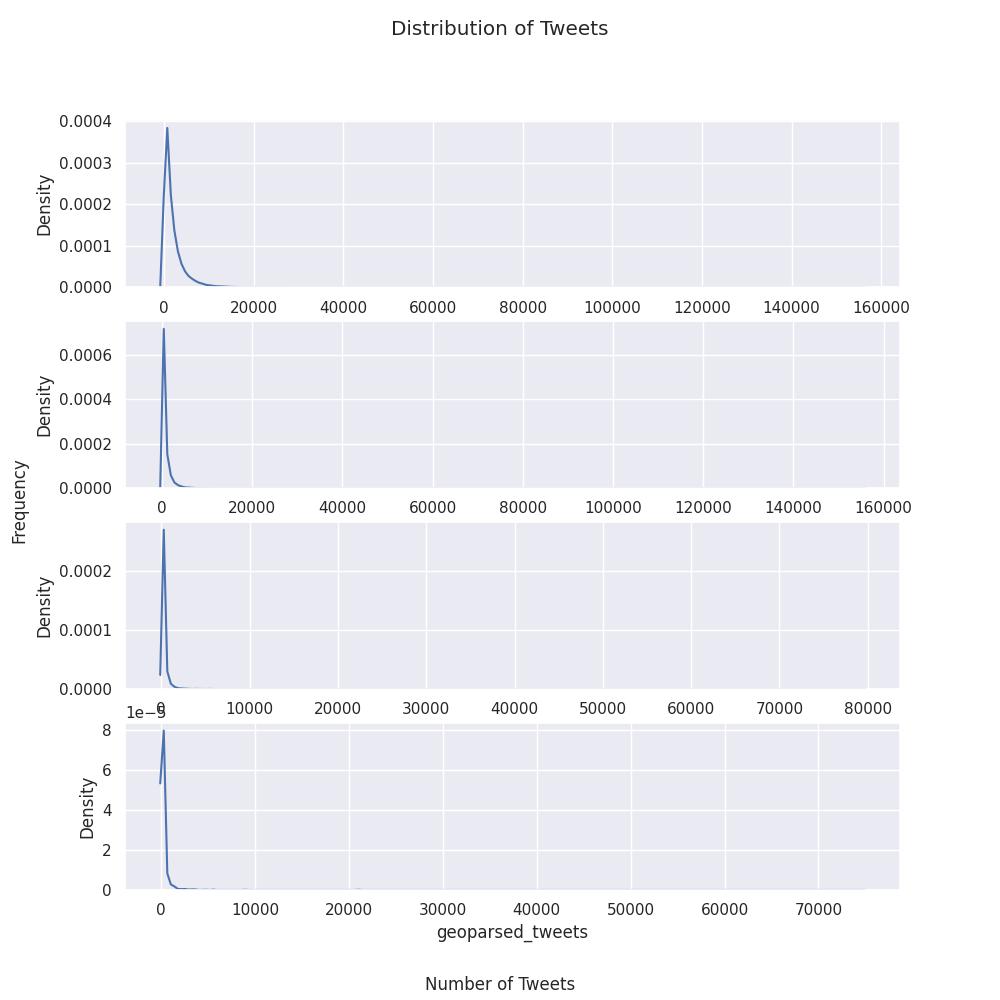
\includegraphics[width=1\textwidth]{images/user_tweets.png}
    
%    \caption{Number of Tweets per User - Total, Geotagged, Mentioned, Geoparsed}
%    \label{fig:user-tweets}
%\end{figure}

The number of users that tweeted only from Argentina was 188 (based on geotag), which is  0.21\% of the total users.

Different types of location information was available for each type of tweet. Mentioned tweets that have been geoparsed have address, city/town, subcountry, country-level granularity based on the output of Google Geolocator API. Geotagged tweets have two main fields for describing location: place name and country. It is difficult to determine how granular the mentioned location is as some place names are counties, while others are names of museums or night clubs, and others still are countries.

\pagebreak
\section{Geotagged}

Geotagged information is not divided into levels of granularity, though it would be possible to determine granularity if geotagged information were geoparsed like the mentioned locations.
Every geotagged tweet has a Place object with attributes name, full name, country and country code. The name is usually a town/city or country, but nothing I could determine that would indicate this granularity. Since the Place object has a country element, it is possible to determine country-level information for downstream analysis.

Geotagged tweets have {\fontfamily{qcr}\selectfont place\_name} and {\fontfamily{qcr}\selectfont place\_country} attributes. 

\subsection{All Countries}

By using the country-level information associated with geotagged tweets, the most geotagged countries were found. Table \ref{table:geotagged-countries}(a) shows the 20 countries with the most number of geotags.


For each user, the countries they geotagged over the course of the relevant time period were found. The 20 most popular geotagged countries are shown in Table \ref{table:geotagged-countries}(b).

\begin{table}
\centering
\begin{subtable}[c]{0.5\textwidth}
\centering
    \begin{tabular}{|c|c|c|}
    \hline
    Location & Number of Tweets & Proportion \\
    \hline
    Argentina & 55743738 & 0.987525 \\
    United States & 152911 & 0.002709 \\
    Brazil & 128727 & 0.002280 \\
    Chile & 68889 & 0.001220 \\
    Uruguay & 55464 & 0.000983 \\
    Spain & 36813 & 0.000652 \\
    Mexico & 30013 & 0.000532 \\
    Paraguay & 29848 & 0.000529 \\
    Colombia & 18635 & 0.000330 \\
    Italy & 15074 & 0.000267 \\
    United Kingdom & 14844 & 0.000263 \\
    Venezuela & 14505 & 0.000257 \\
    Ecuador & 13178 & 0.000233 \\
    France & 12456 & 0.000221 \\
    Russia & 9022 & 0.000160 \\
    Peru & 8327 & 0.000148 \\
    Germany & 6775 & 0.000120 \\
    Japan & 5729 & 0.000101 \\
    Dominican Republic & 5140 & 0.000091 \\
    Canada & 5104 & 0.000090 \\
    Other & 67692 & 0.001199 \\
    \hline
    \end{tabular}
\subcaption{in Tweets}
\end{subtable}

\begin{subtable}[c]{0.5\textwidth}
\centering
    \begin{tabular}{|c|c|c|}
    \hline
    Location & Number of Tweets & Proportion \\
    \hline
    Argentina & 89329 & 0.723072 \\
    Brazil & 6008 & 0.048632 \\
    United States & 5410 & 0.043791 \\
    Chile & 2970 & 0.024041 \\
    Uruguay & 2113 & 0.017104 \\
    Mexico & 1693 & 0.013704 \\
    Spain & 1681 & 0.013607 \\
    Italy & 1017 & 0.008232 \\
    Peru & 959 & 0.007763 \\
    United Kingdom & 939 & 0.007601 \\
    Paraguay & 938 & 0.007593 \\
    France & 883 & 0.007147 \\
    Colombia & 788 & 0.006378 \\
    Dominican Republic & 444 & 0.003594 \\
    Germany & 429 & 0.003473 \\
    The Netherlands & 402 & 0.003254 \\
    Ecuador & 393 & 0.003181 \\
    Japan & 280 & 0.002266 \\
    Venezuela & 267 & 0.002161 \\
    Panama & 266 & 0.002153 \\
    Other & 6332 & 0.051254 \\
    \hline
    \end{tabular}
\caption{by Users}
\end{subtable}
\caption{Most Commonly Geotagged Countries}
\label{table:geotagged-countries}
\end{table}

For the top 5 most geotagged countries in Table \ref{table:geotagged-countries} (excluding Argentina), the number of tweets and the number of users geotagging those countries was was found for each epi week (see Figure \ref{fig:geotagged-countries-tweets-epi-week} and Figure \ref{fig:geotagged-countries-users-epi-week}).

%\begin{figure}[H]
%        \centering
\begin{figure}[H]%{.49\linewidth}
    \centering
    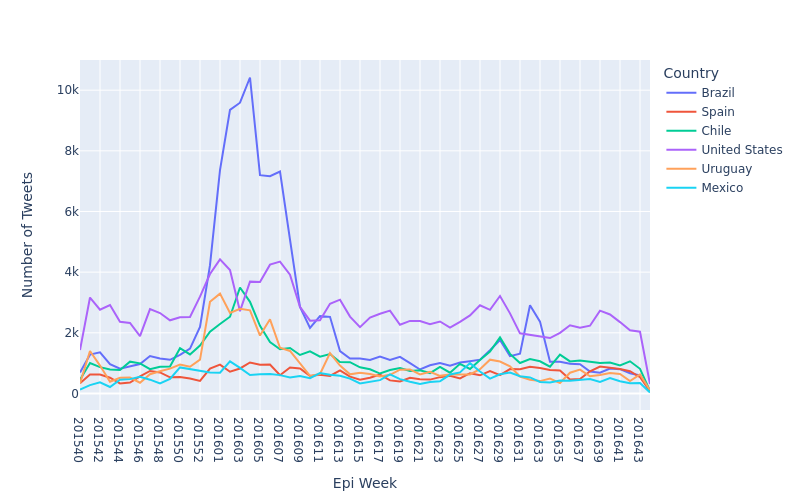
\includegraphics[width=1\textwidth]{images/geotagged_tweets_country_epi_week.png}
    \caption{by Tweets}
    \label{fig:geotagged-countries-tweets-epi-week}
\end{figure}
%        \hfill


\begin{figure}[H]%{.49\linewidth}
    \centering
    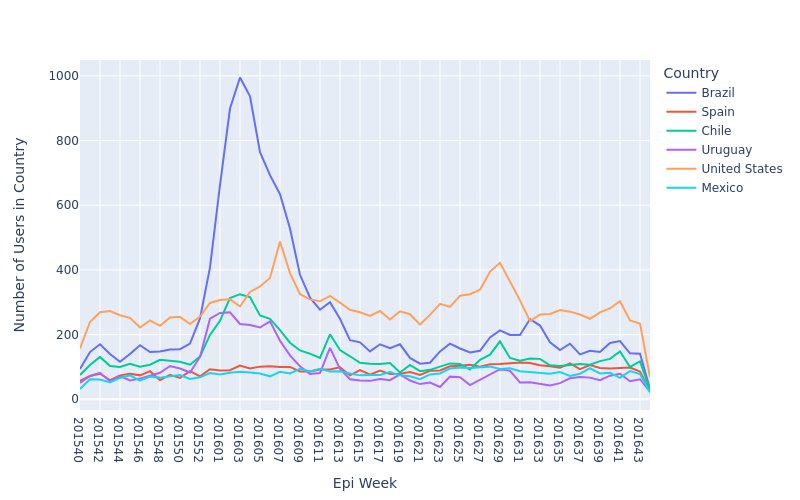
\includegraphics[width=1\textwidth]{images/geotagged_users_country_epi_week.png}
    \caption{by User}
    \label{fig:geotagged-countries-users-epi-week}
\end{figure}
%        \caption{Distribution of Most Geotagged Countries}
%        \label{fig:geotagged-countries-epi-week}
%\end{figure}

%Figure \ref{fig:mentioned-tweets-argentina-epi-week} shows the number of times Argentina was mentioned in tweets during each epi week.

\subsection{Argentina}

By considering {\fontfamily{qcr}\selectfont place\_name}, the the most commonly geotagged locations in tweets in Argentina were found (see Table \ref{table:mentioned-argentina}(a). Similarly, the most commonly geotagged locations by users in Argentina are shown in Table \ref{table:mentioned-argentina}(b).

\begin{table}
\centering
\begin{subtable}[c]{0.5\textwidth}
\centering
    \begin{tabular}{|c|c|c|}
    \hline
    Location & Number of Tweets & Proportion \\
    \hline
    Ciudad Autónoma de Buenos Aires & 6013615 & 0.107880 \\
    Córdoba & 4963649 & 0.089044 \\
    Buenos Aires & 3530325 & 0.063331 \\
    La Plata & 1824224 & 0.032725 \\
    Rosario & 1787751 & 0.032071 \\
    Santa Fe & 1258011 & 0.022568 \\
    Mar del Plata & 1136730 & 0.020392 \\
    Entre Ríos & 1108310 & 0.019882 \\
    Corrientes & 1076449 & 0.019311 \\
    Neuquén & 913416 & 0.016386 \\
    Lomas de Zamora & 806670 & 0.014471 \\
    Río Negro & 786264 & 0.014105 \\
    Bahía Blanca & 751970 & 0.013490 \\
    Santa Fé & 742449 & 0.013319 \\
    Lanús Oeste & 735798 & 0.013200 \\
    Almirante Brown & 700483 & 0.012566 \\
    Quilmes & 697071 & 0.012505 \\
    González Catán & 687619 & 0.012335 \\
    Mendoza & 657052 & 0.011787 \\
    Ciudad del Libertador General San Martín & 602969 & 0.010817 \\
    Other & 24361219 & 0.437022 \\
    \hline
    \end{tabular}
\subcaption{in Tweets}
\end{subtable}
\begin{subtable}[c]{0.5\textwidth}
\centering
    \begin{tabular}{|c|c|c|}
    \hline
    Location & Number of Tweets & Proportion \\
    \hline
    Ciudad Autónoma de Buenos Aires & 40660 & 0.093223 \\
    Buenos Aires & 31355 & 0.071889 \\
    Córdoba & 18180 & 0.041682 \\
    Villa Soldati & 9549 & 0.021893 \\
    Santa Fe & 9251 & 0.021210 \\
    La Plata & 9196 & 0.021084 \\
    Rosario & 8842 & 0.020272 \\
    Mar del Plata & 7868 & 0.018039 \\
    Entre Ríos & 7867 & 0.018037 \\
    San Isidro & 7216 & 0.016544 \\
    Tigre & 7098 & 0.016274 \\
    Avellaneda & 6644 & 0.015233 \\
    Vicente López & 6390 & 0.014651 \\
    González Catán & 6357 & 0.014575 \\
    Argentina & 6252 & 0.014334 \\
    Ciudad del Libertador General San Martín & 6132 & 0.014059 \\
    Morón & 5888 & 0.013500 \\
    Lomas de Zamora & 5577 & 0.012787 \\
    Caseros & 5244 & 0.012023 \\
    Buenos Aires City Region & 4966 & 0.011386 \\
    Other & 225628 & 0.517306 \\
    \hline
    \end{tabular}
\caption{by Users}
\end{subtable}
\caption{Most Commonly Geotagged Locations in Argentina}
\label{table:geotagged-argentina}
\end{table}

The distribution of tweets geotagged with Argentina over the course of the relevant time period is shown in Figure \ref{fig:geotagged-tweets-argentina-epi-week}

\begin{figure}[H]
    \centering
    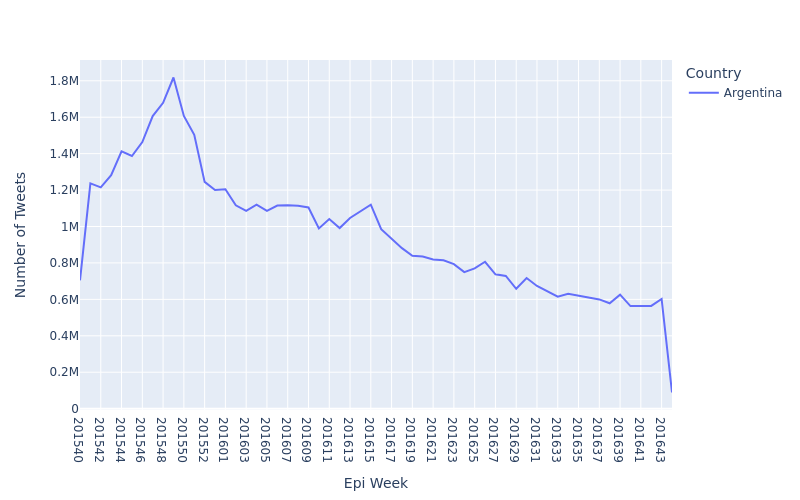
\includegraphics[width=1\textwidth]{images/geotagged_tweets_argentina_epi_week.png}
    
    \caption{Distribution of Geotagged Tweets with Argentina}
    \label{fig:geotagged-tweets-argentina-epi-week}
\end{figure}

\subsection{USA}

By considering {\fontfamily{qcr}\selectfont place\_name}, the the most commonly geotagged locations in tweets in USA were found (see Table \ref{table:mentioned-argentina}(a). Similarly, the most commonly geotagged locations by users in USA are shown in Table \ref{table:mentioned-argentina}(b).

\begin{table}
\centering
\begin{subtable}[c]{0.5\textwidth}
\centering
    \begin{tabular}{|c|c|c|}
    \hline
    Location & Number of Tweets & Proportion \\
    \hline
    Manhattan & 13989 & 0.091516 \\
    United States & 13751 & 0.089959 \\
    New York & 11383 & 0.074468 \\
    Florida & 10991 & 0.071903 \\
    Alaska & 9713 & 0.063543 \\
    Miami Beach & 9235 & 0.060416 \\
    California & 7967 & 0.052120 \\
    Miami & 4486 & 0.029347 \\
    Buenos Aires & 3165 & 0.020705 \\
    North Carolina & 3124 & 0.020437 \\
    Orlando & 2929 & 0.019162 \\
    Paterson & 2487 & 0.016270 \\
    Los Angeles & 2411 & 0.015773 \\
    Nevada & 2279 & 0.014909 \\
    Brooklyn & 2128 & 0.013921 \\
    Hawaii & 2045 & 0.013378 \\
    Washington & 1967 & 0.012868 \\
    San Francisco & 1779 & 0.011638 \\
    Hollywood & 1603 & 0.010487 \\
    Oklahoma & 1331 & 0.008707 \\
    Other & 42858 & 0.280378 \\
    \hline
    \end{tabular}
\subcaption{in Tweets}
\end{subtable}

\begin{subtable}[c]{0.5\textwidth}
\centering
    \begin{tabular}{|c|c|c|}
    \hline
    Location & Number of Tweets & Proportion \\
    \hline
    Florida & 1294 & 0.076855 \\
    Miami Beach & 1226 & 0.072816 \\
    Manhattan & 1040 & 0.061769 \\
    Miami & 946 & 0.056186 \\
    Orlando & 709 & 0.042110 \\
    New York & 417 & 0.024767 \\
    Los Angeles & 389 & 0.023104 \\
    United States & 350 & 0.020788 \\
    Brooklyn & 257 & 0.015264 \\
    Queens & 227 & 0.013482 \\
    San Francisco & 196 & 0.011641 \\
    California & 192 & 0.011403 \\
    Hollywood & 163 & 0.009681 \\
    Sunny Isles Beach & 163 & 0.009681 \\
    Paradise & 161 & 0.009562 \\
    Washington & 156 & 0.009265 \\
    Fort Lauderdale & 156 & 0.009265 \\
    Las Vegas & 152 & 0.009028 \\
    Doral & 129 & 0.007662 \\
    Chicago & 118 & 0.007008 \\
    Other & 8396 & 0.498664 \\
    \hline
    \end{tabular}
\caption{by Users}
\end{subtable}
\caption{Most Commonly Geotagged Locations in USA}
\label{table:geotagged-usa}
\end{table}



\begin{figure}[H]
    \centering
    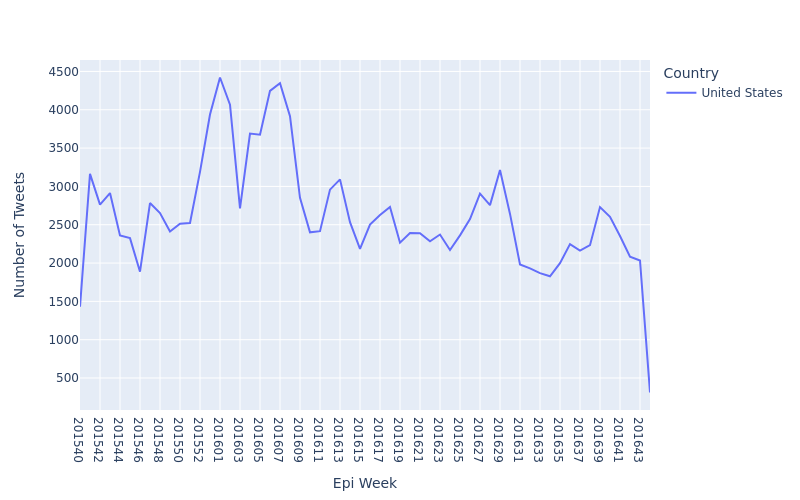
\includegraphics[width=1\textwidth]{images/geotagged_tweets_usa_epi_week.png}
    
    \caption{Distribution of Tweets Geotagged with USA}
    \label{fig:geotagged-tweets-usa-epi-week}
\end{figure}

\subsection{Brazil}

By considering {\fontfamily{qcr}\selectfont place\_name}, the the most commonly geotagged locations in tweets in Brazil were found (see Table \ref{table:mentioned-argentina}(a). Similarly, the most commonly geotagged locations by users in Brazil are shown in Table \ref{table:mentioned-argentina}(b).


\begin{table}
\centering
\begin{subtable}[c]{0.5\textwidth}
\centering
    \begin{tabular}{|c|c|c|}
    \hline
    Location & Number of Tweets & Proportion \\
    \hline
    Florianópolis & 23620 & 0.183489 \\
    Rio de Janeiro & 17070 & 0.132606 \\
    Bombinhas & 12285 & 0.095435 \\
    Ananindeua & 8702 & 0.067600 \\
    Balneário Camboriú & 5449 & 0.042330 \\
    Sao Paulo & 5069 & 0.039378 \\
    Foz do Iguaçu & 4787 & 0.037187 \\
    Itapema & 4393 & 0.034126 \\
    Armação dos Búzios & 2785 & 0.021635 \\
    Ipanema & 2399 & 0.018636 \\
    Cuiabá & 1796 & 0.013952 \\
    Porto Alegre & 1766 & 0.013719 \\
    São Vicente & 1151 & 0.008941 \\
    Natal & 1087 & 0.008444 \\
    São Sebastião & 1082 & 0.008405 \\
    Torres & 1032 & 0.008017 \\
    Mata de São João & 1014 & 0.007877 \\
    Rio Grande do Sul & 909 & 0.007061 \\
    Porto Seguro & 892 & 0.006929 \\
    Salvador & 892 & 0.006929 \\
    Other & 29667 & 0.230464 \\
    \hline
    \end{tabular}
\subcaption{in Tweets}
\end{subtable}

\begin{subtable}[c]{0.5\textwidth}
\centering
    \begin{tabular}{|c|c|c|}
    \hline
    Location & Number of Tweets & Proportion \\
    \hline
    Florianópolis & 1140 & 0.096178 \\
    Rio de Janeiro & 1032 & 0.087067 \\
    Foz do Iguaçu & 701 & 0.059141 \\
    Bombinhas & 627 & 0.052898 \\
    Balneário Camboriú & 464 & 0.039146 \\
    Sao Paulo & 383 & 0.032312 \\
    Armação dos Búzios & 296 & 0.024973 \\
    Guarulhos & 285 & 0.024045 \\
    Itapema & 283 & 0.023876 \\
    Santa Catarina & 166 & 0.014005 \\
    São Gabriel & 159 & 0.013414 \\
    Uruguaiana & 137 & 0.011558 \\
    Torres & 128 & 0.010799 \\
    Salvador & 126 & 0.010630 \\
    Porto Seguro & 123 & 0.010377 \\
    Porto Alegre & 119 & 0.010040 \\
    Angra dos Reis & 117 & 0.009871 \\
    Brazil & 115 & 0.009702 \\
    Garopaba & 107 & 0.009027 \\
    Brasília & 103 & 0.008690 \\
    Other & 5242 & 0.442251 \\
    \hline
    \end{tabular}
\caption{by Users}
\end{subtable}
\caption{Most Commonly Geotagged Locations in Brazil}
\label{table:geotagged-brazil}
\end{table}


\begin{figure}[H]
    \centering
    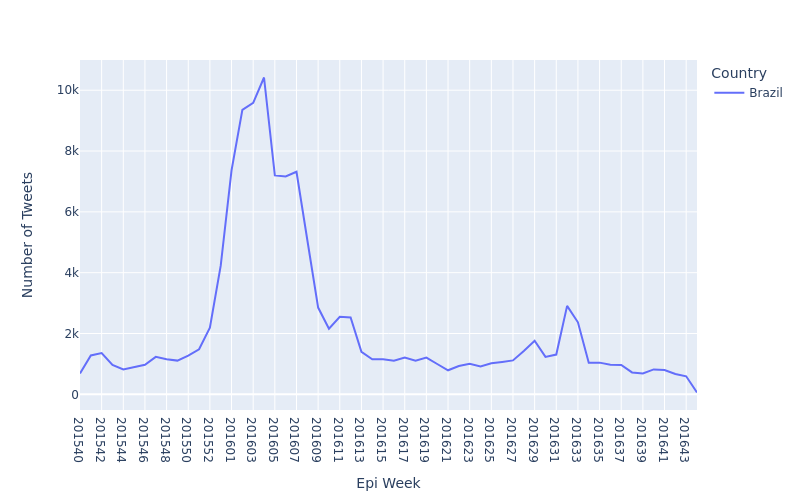
\includegraphics[width=1\textwidth]{images/geotagged_tweets_brazil_epi_week.png}
    
    \caption{Distribution of Tweets Geotagged with Brazil}
    \label{fig:geotagged-tweets-brazil-epi-week}
\end{figure}

\pagebreak

\section{Mentioned}

Since some tweets mentioned more than one location, the total number of toponyms (LOC mentions) was 9,017,197 (tweets duplicated to capture all mentions), compared to 7,269,062 mentioned tweets. Similarly, the number of geoparsed toponyms was 4,139,502, compared to 3,462,888 geoparsed tweets. This section explores geoparsed toponyms, as they have the most location information associated with them.

514284 locations were disregarded (corresponding to 828684 tweets), 46952 were kept (corresponding to 7204497 tweets). 

 
\subsection{Granularity}

Figure \ref{fig:mention-pie} shows the granularity of geoparsed toponyms. 

\begin{figure}[H]
    \centering
    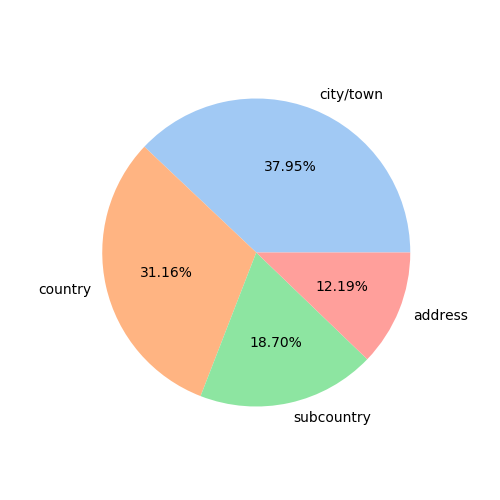
\includegraphics[width=0.5\textwidth]{images/granularity.png}
    
    \caption{Granularity of Mentions}
    \label{fig:mention-pie}
\end{figure}

%Table \ref{tab:granularity} shows the tweet granularity of mentions within tweets, excluding those that did not correspond to a location in Geolocator API.
The "subcountry" granularity was used to describe geoparsed toponyms that contained a county, province, region, district etc. but did not contain a city/town. "Address" was used to describe a toponym that had a specific street-level address.

\begin{comment}
\begin{table}[H]
  \centering
  \begin{tabular}{|c|c|c|}
    \hline
    %& \multicolumn{2}{c|}{\textbf{Mention}} & \multicolumn{2}{c|}{\textbf{Mention Only}} \\
    %\cline{3-6}
    \textbf{Granularity} & \textbf{Number of Tweets} & \textbf{Proportion}\\
    \hline
    city/town &	1570867 &	0.379482 \\
    \hline
    country &	1290046 &	0.311643 \\
    \hline
    subcountry &	773963 &	0.186970 \\
    address & 	504626 & 	0.121905 \\
    \hline
  \end{tabular}
  \caption{Geoparsed Toponym Granularity}
  \label{tab:granularity}
\end{table}
\end{comment}

\subsection{All Countries}

To understand which countries were mentioned most often in tweets, the number of geoparsed toponyms associated with each mentioned country was found. The top 20 countries mentioned in tweets are shown in Table \ref{table:mentioned-countries}(a).

For each user, a list of countries they mentioned during the relevant time period was found (using location information from geoparsed toponyms). This information was aggregated by finding the number of users that mentioned each country. Table \ref{table:mentioned-countries}(b) shows the top 20 countries mentioned most often by users.

\begin{table}[H]
\begin{subtable}[c]{0.5\textwidth}
\centering
\begin{tabular}{|c|c|c|}
\hline
    \textbf{Location} & \textbf{Count} & \textbf{Proportion} \\
    \hline
    Argentina & 2157309.0 & 0.521152 \\
    USA & 532081.0 & 0.128537 \\
    Brazil & 131189.0 & 0.031692 \\
    Chile & 97427.0 & 0.023536 \\
    Spain & 96466.0 & 0.023304 \\
    Italy & 94749.0 & 0.022889 \\
    France & 71005.0 & 0.017153 \\
    Mexico & 69886.0 & 0.016883 \\
    United States & 67970.0 & 0.016420 \\
    Colombia & 48817.0 & 0.011793 \\
    Venezuela & 40560.0 & 0.009798 \\
    Uruguay & 39403.0 & 0.009519 \\
    UK & 38552.0 & 0.009313 \\
    Puerto Rico & 28763.0 & 0.006948 \\
    Japan & 27415.0 & 0.006623 \\
    China & 25588.0 & 0.006181 \\
    Germany & 23716.0 & 0.005729 \\
    Paraguay & 22557.0 & 0.005449 \\
    Bulgaria & 21419.0 & 0.005174 \\
    Peru & 21268.0 & 0.005138 \\
    Other & 464182.0 & 0.112135 \\
    \hline
    \end{tabular}
\subcaption{in Tweets}
%\label{table:mentioned-countries-tweets}
\end{subtable}
\begin{subtable}[c]{0.5\textwidth}
\centering
\begin{tabular}{|c|c|c|}
\hline
    \textbf{Location} & \textbf{Count} & \textbf{Proportion} \\
    \hline
    Argentina & 74323 & 0.123 \\
    USA & 60282 & 0.100 \\
    Brazil & 28767 & 0.048 \\
    Italy & 27548 & 0.046 \\
    Spain & 24842 & 0.041 \\
    Chile & 22576 & 0.037 \\
    France & 22121 & 0.037 \\
    Mexico & 19505 & 0.032 \\
    United States & 14443 & 0.024 \\
    Colombia & 12920 & 0.021 \\
    UK & 12052 & 0.020 \\
    Uruguay & 10966 & 0.018 \\
    China & 10515 & 0.017 \\
    Japan & 8890 & 0.015 \\
    Germany & 8575 & 0.014 \\
    Venezuela & 8212 & 0.014 \\
    Puerto Rico & 8209 & 0.014 \\
    Australia & 8066 & 0.013 \\
    Peru & 7907 & 0.013 \\
    India & 7741 & 0.013 \\
    Other & 205642 & 0.340 \\
    \hline
    \end{tabular}
\subcaption{by Users}
\label{table:mentioned-countries}
\end{subtable}
\caption{Most Mentioned Countries}
\end{table}

To investigate temporal patterns, the number of times the top 5 countries in \ref{table:mentioned-countries}(a) (excluding Argentina) were mentioned during each epi week was found. Figure \ref{fig:mentioned-tweets-country-epi-week} shows when these countries were mentioned over time.

Similarly, the number of users mentioning the top 5 countries in \ref{table:mentioned-countries}(b) (excluding Argentina) during each epi week was found (see Figure \ref{fig:mentioned-users-country-epi-week}).

\begin{figure}[H]
    \centering
    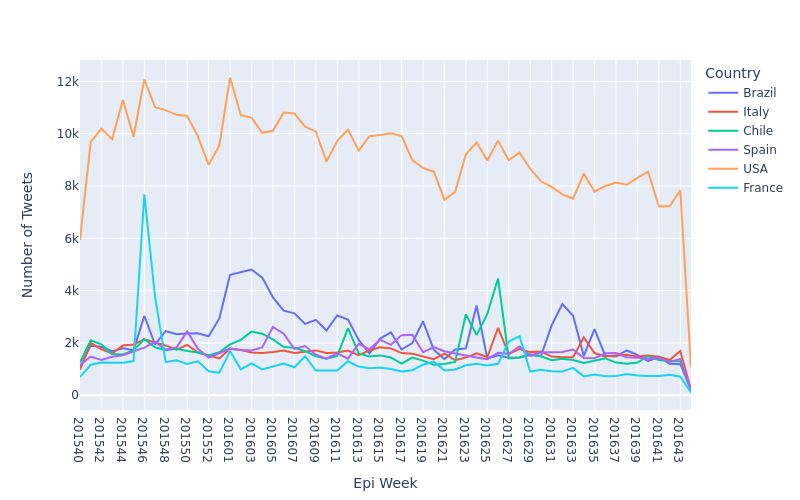
\includegraphics[width=1\textwidth]{images/mentioned_tweets_country_epi_week.png}
    
    \caption{Distribution of Top 5 Most Geotagged Countries (Tweets)}
    \label{fig:mentioned-tweets-country-epi-week}
\end{figure}

\begin{figure}[H]
    \centering
    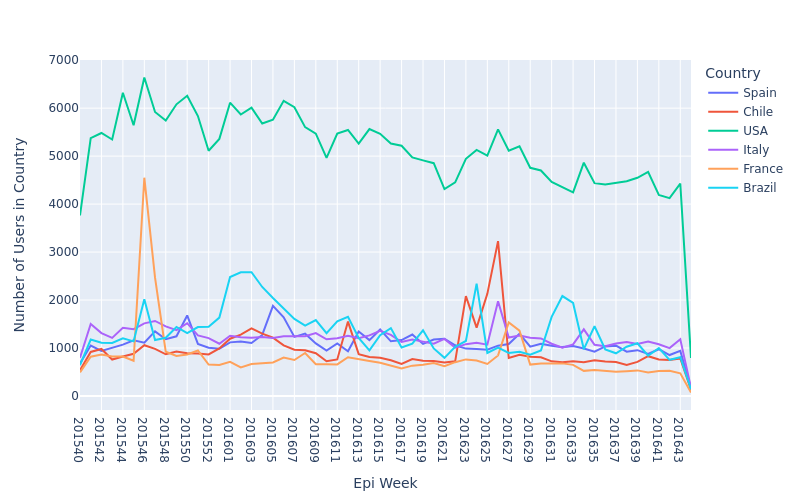
\includegraphics[width=1\textwidth]{images/mentioned_users_country_epi_week.png}
    
    \caption{Distribution of Top 5 Most Geotagged Countries (Users)}
    \label{fig:mentioned-users-country-epi-week}
\end{figure}

\subsection{Argentina}

If geoparsed toponyms contained city/town information, the most commonly mentioned cities/towns in tweets in Argentina were found (see Table \ref{table:mentioned-argentina}(a).
Similarly, the most commonly mentioned cities/towns in Argentina are shown in Table \ref{table:mentioned-argentina}(b).
Figure \ref{fig:mentioned-tweets-argentina-epi-week} shows the number of times Argentina was mentioned in tweets during each epi week.

\begin{table}
\centering
\begin{subtable}[c]{0.5\textwidth}
\centering
\begin{tabular}{|c|c|c|}
\hline
    \textbf{Location} & \textbf{Count} & \textbf{Proportion} \\
    \hline
    Rosario & 88325.0 & 0.086508 \\
    San Carlos de Bariloche & 53501.0 & 0.052400 \\
    La Plata & 46432.0 & 0.045477 \\
    Capital Department & 43428.0 & 0.042535 \\
    Mar del Plata & 42159.0 & 0.041292 \\
    Salta & 37853.0 & 0.037074 \\
    San Miguel de Tucumán & 31238.0 & 0.030595 \\
    Quilmes & 21652.0 & 0.021207 \\
    Avellaneda & 16396.0 & 0.016059 \\
    San Salvador de Jujuy & 14388.0 & 0.014092 \\
    Posadas & 12154.0 & 0.011904 \\
    San Martín & 11944.0 & 0.011698 \\
    Catamarca & 11856.0 & 0.011612 \\
    Bahía Blanca & 11609.0 & 0.011370 \\
    Av. Hipólito Yrigoyen s/n & 10619.0 & 0.010401 \\
    Ezeiza & 9584.0 & 0.009387 \\
    San Isidro & 9092.0 & 0.008905 \\
    Villa Carlos Paz & 9079.0 & 0.008892 \\
    Ushuaia & 8644.0 & 0.008466 \\
    Puerto Madero & 8583.0 & 0.008406 \\
    Other & 514462.0 & 0.503880 \\
    \hline
    \end{tabular}
\subcaption{in Tweets}
\end{subtable}

\begin{subtable}[c]{0.5\textwidth}
\centering
\begin{tabular}{|c|c|c|}
\hline
    \textbf{Location} & \textbf{Count} & \textbf{Proportion} \\
    \hline
    San Carlos de Bariloche & 15330.0 & 0.056753 \\
    Rosario & 11999.0 & 0.044421 \\
    Capital Department & 8259.0 & 0.030575 \\
    Mar del Plata & 8187.0 & 0.030309 \\
    La Plata & 7369.0 & 0.027280 \\
    Avellaneda & 5643.0 & 0.020891 \\
    Quilmes & 5566.0 & 0.020606 \\
    San Miguel de Tucumán & 5521.0 & 0.020439 \\
    Salta & 5343.0 & 0.019780 \\
    San Martín & 4137.0 & 0.015315 \\
    San Salvador de Jujuy & 3919.0 & 0.014508 \\
    Puerto Madero & 3826.0 & 0.014164 \\
    Ezeiza & 3427.0 & 0.012687 \\
    Av. Hipólito Yrigoyen s/n & 3378.0 & 0.012506 \\
    Villa Carlos Paz & 3377.0 & 0.012502 \\
    Tandil & 3027.0 & 0.011206 \\
    San Isidro & 2534.0 & 0.009381 \\
    Santiago del Estero & 2434.0 & 0.009011 \\
    Recoleta & 2293.0 & 0.008489 \\
    Catamarca & 2249.0 & 0.008326 \\
    Other & 162302.0 & 0.600851 \\
    \hline
    \end{tabular}
\caption{by Users}
\end{subtable}
\caption{Most Commonly Mentioned cities/towns in Argentina}
\label{table:mentioned-argentina}
\end{table}

\begin{figure}[H]
    \centering
    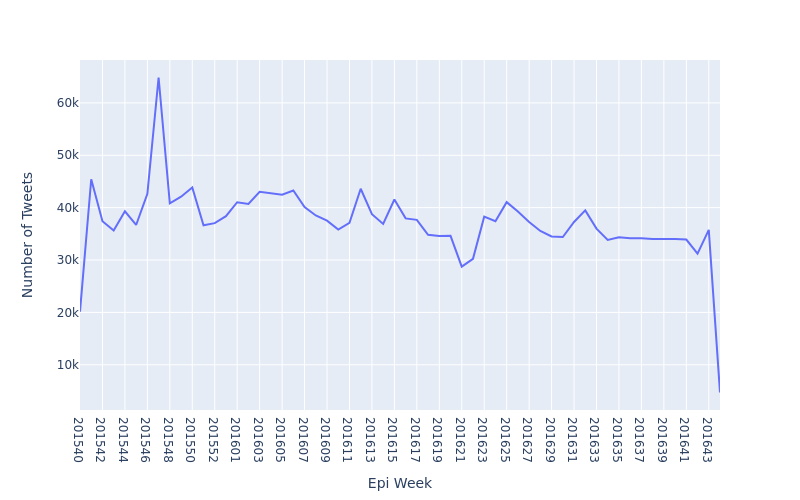
\includegraphics[width=1\textwidth]{images/mentioned_tweets_argentina_epi_week.png}
    
    \caption{Tweets Mentioning Argentina Over Time}
    \label{fig:mentioned-tweets-argentina-epi-week}
\end{figure}

\subsection{USA}

If geoparsed toponyms contained city/town information, the most commonly mentioned cities/towns in tweets in USA were found (see Table \ref{table:mentioned-argentina}(a).
Similarly, the most commonly mentioned cities/towns in USA are shown in Table \ref{table:mentioned-argentina}(b).
Figure \ref{fig:mentioned-tweets-argentina-epi-week} shows the number of times USA was mentioned in tweets during each epi week.

USA was chosen because it was the second most mentioned country from previous analysis.

\begin{table}
\centering
\begin{subtable}[c]{0.5\textwidth}
\centering
\begin{tabular}{|c|c|c|}
\hline
    \textbf{Location} & \textbf{Count} & \textbf{Proportion} \\
    \hline
    Santa Fe & 48704.0 & 0.181962 \\
    New York & 22526.0 & 0.084159 \\
    Miami & 17731.0 & 0.066244 \\
    Santa Cruz & 13279.0 & 0.049611 \\
    Santa Rosa & 10286.0 & 0.038429 \\
    Los Angeles & 9557.0 & 0.035706 \\
    San Francisco & 9056.0 & 0.033834 \\
    Chicago & 8632.0 & 0.032250 \\
    San Rafael & 4986.0 & 0.018628 \\
    Atlanta & 4765.0 & 0.017802 \\
    Brooklyn & 4664.0 & 0.017425 \\
    Orlando & 4370.0 & 0.016327 \\
    San Fernando & 4284.0 & 0.016005 \\
    San Nicolas Island & 3950.0 & 0.014758 \\
    Las Vegas & 3624.0 & 0.013540 \\
    Miramar & 2887.0 & 0.010786 \\
    Miami Beach & 2853.0 & 0.010659 \\
    San Jose & 2744.0 & 0.010252 \\
    Martinez & 2544.0 & 0.009505 \\
    Buena & 2461.0 & 0.009195 \\
    Other & 81363.0 & 0.303979 \\
    \hline
    \end{tabular}
\subcaption{in Tweets}
\end{subtable}

\begin{subtable}[c]{0.5\textwidth}
\centering
\begin{tabular}{|c|c|c|}
\hline
    \textbf{Location} & \textbf{Count} & \textbf{Proportion} \\
    \hline
    Santa Fe & 8523.0 & 0.094506 \\
    Miami & 7605.0 & 0.084327 \\
    New York & 5883.0 & 0.065233 \\
    Los Angeles & 3586.0 & 0.039763 \\
    Santa Cruz & 2889.0 & 0.032034 \\
    Chicago & 2870.0 & 0.031823 \\
    Santa Rosa & 2488.0 & 0.027588 \\
    Orlando & 2334.0 & 0.025880 \\
    San Francisco & 2232.0 & 0.024749 \\
    Alta & 1864.0 & 0.020669 \\
    Las Vegas & 1791.0 & 0.019859 \\
    Buena & 1546.0 & 0.017143 \\
    Islandia & 1429.0 & 0.015845 \\
    Brooklyn & 1264.0 & 0.014016 \\
    Miramar & 1153.0 & 0.012785 \\
    Atlanta & 1151.0 & 0.012763 \\
    San Pablo & 1140.0 & 0.012641 \\
    San Jose & 1118.0 & 0.012397 \\
    San Nicolas Island & 1115.0 & 0.012363 \\
    San Antonio & 1110.0 & 0.012308 \\
    Other & 37094.0 & 0.411310 \\
    \hline
    \end{tabular}
\caption{by Users}
\end{subtable}
\caption{Most Commonly Mentioned cities/towns in USA}
\label{table:mentioned-usa}
\end{table}

\begin{figure}[H]
    \centering
    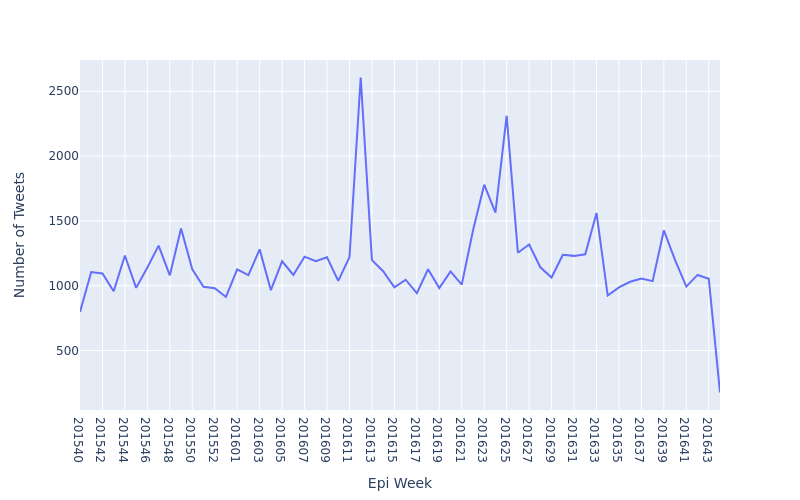
\includegraphics[width=1\textwidth]{images/mentioned_tweets_us_epi_week.png}
    
    \caption{Tweets Mentioning USA Over Time}
    \label{fig:mentioned-tweets-us-epi-week}
\end{figure}

\subsection{Brazil}

If geoparsed toponyms contained city/town information, the most commonly mentioned cities/towns in tweets in USA were found (see Table \ref{table:mentioned-argentina}(a).
Similarly, the most commonly mentioned cities/towns in USA are shown in Table \ref{table:mentioned-argentina}(b).
Figure \ref{fig:mentioned-tweets-argentina-epi-week} shows the number of times USA was mentioned in tweets during each epi week.

Brazil was chosen because it was third most mentioned country and it has the highest incidence of dengue virus in the Americas.

\begin{table}
\centering
\begin{subtable}[c]{0.5\textwidth}
\centering
\begin{tabular}{|c|c|c|}
\hline
    \textbf{Location} & \textbf{Count} & \textbf{Proportion} \\
    \hline
    Brasília - Brasilia & 6431.0 & 0.164830 \\
    Ananindeua & 5934 & 0.152091 \\
    Rio de Janeiro & 4205.0 & 0.107776 \\
    São Paulo & 2454.0 & 0.062897 \\
    Florianópolis & 2050.0 & 0.052543 \\
    Manaus & 926.0 & 0.023734 \\
    Armação dos Búzios & 668.0 & 0.017121 \\
    Av. Brasil & 571.0 & 0.014635 \\
    Foz do Iguaçu & 539.0 & 0.013815 \\
    State of São Paulo & 510.0 & 0.013072 \\
    Rio de Janeiro - RJ & 506.0 & 0.012969 \\
    Santa Catarina & 467.0 & 0.011969 \\
    São Paulo - SP & 455.0 & 0.011662 \\
    Porto Alegre & 432.0 & 0.011072 \\
    Belo Horizonte & 403.0 & 0.010329 \\
    Praia de Canasvieiras & 400.0 & 0.010252 \\
    Curitiba & 387.0 & 0.009919 \\
    SC & 354.0 & 0.009073 \\
    Palmas & 352.0 & 0.009022 \\
    Maracanã & 328.0 & 0.008407 \\
    Other & 10323.0 & 0.264584 \\
    \hline
    \end{tabular}
\subcaption{in Tweets}
\end{subtable}

\begin{subtable}[c]{0.5\textwidth}
\centering
\begin{tabular}{|c|c|c|}
\hline
    \textbf{Location} & \textbf{Count} & \textbf{Proportion} \\
    \hline
    Rio de Janeiro & 1753.0 & 0.121770 \\
    Brasília - Brasilia & 1724.0 & 0.119755 \\
    Florianópolis & 876.0 & 0.060850 \\
    São Paulo & 860.0 & 0.059739 \\
    Manaus & 782.0 & 0.054321 \\
    Av. Brasil & 369.0 & 0.025632 \\
    Rio de Janeiro - RJ & 309.0 & 0.021464 \\
    State of São Paulo & 297.0 & 0.020631 \\
    Armação dos Búzios & 288.0 & 0.020006 \\
    Palmas & 269.0 & 0.018686 \\
    Maracanã & 251.0 & 0.017435 \\
    Foz do Iguaçu & 242.0 & 0.016810 \\
    Porto Alegre & 233.0 & 0.016185 \\
    Santa Catarina & 217.0 & 0.015074 \\
    Belo Horizonte & 185.0 & 0.012851 \\
    Ipanema & 167.0 & 0.011600 \\
    State of Santa Catarina & 165.0 & 0.011462 \\
    Praia de Canasvieiras & 164.0 & 0.011392 \\
    Curitiba & 156.0 & 0.010836 \\
    Praia dos Ingleses & 153.0 & 0.010628 \\
    Other & 4936.0 & 0.342873 \\
    \hline
    \end{tabular}
\caption{by Users}
\end{subtable}
\caption{Most Commonly Mentioned cities/towns in Brazil}
\label{table:mentioned-brazil}
\end{table}

\begin{figure}[H]
    \centering
    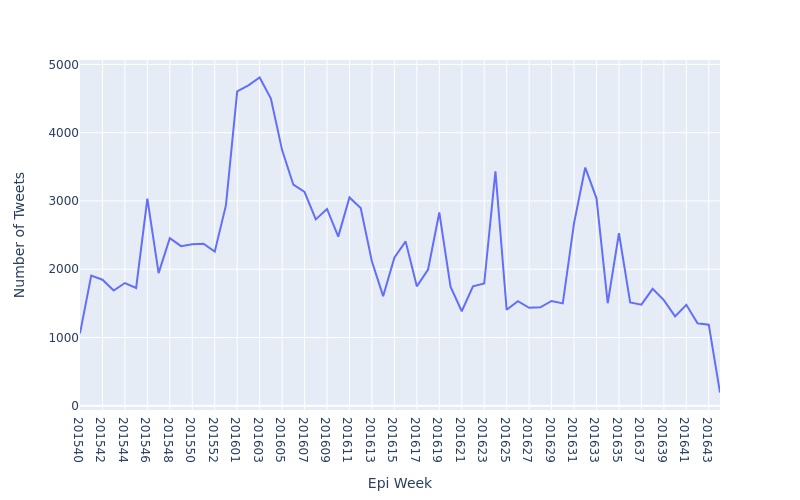
\includegraphics[width=1\textwidth]{images/mentioned_tweets_br_epi_week.png}
    
    \caption{Tweets Mentioning Brazil Over Time}
    \label{fig:mentioned-tweets-br-epi-week}
\end{figure}

\pagebreak
\section{Geotagged \& Mentioned}

Where a tweet had both a geoparsed set of coordinates and a geotagged set of coordinates, the geodesic distance was calculated in kilometres.

A subset of these tweets had more than one geoparsed set of coordinates. These tweets were called Duplicates. The subset of tweets with a unique geoparsed set of coordinates was called Non-Duplicates. 

Table \ref{table:summary-distances} shows summary statistics for distances between geotagged coordinates and mentioned (geoparsed) coordinates for all the tweets with geoparsed and geotagged locations, as well as subsets Duplicates and Non-Duplicates.

\begin{table}[H]
    \centering
    \begin{tabular}{|l|c|c|c|}
    \hline
    Metric & All & Duplicates & Non-Duplicates \\
    \hline
    MdnED & 479.11 & 142.58 & 631.54 \\
    MED & 2708.79 & 1977.22 & 3477.69 \\
    Accuracy@0.1 & 0.031 & 0.033 & 0.028 \\
    Accuracy@0.5 & 0.074 & 0.080 & 0.066 \\
    Accuracy@1 & 0.132 & 0.140 & 0.124 \\
    Accuracy@5 & 0.254 & 0.306 & 0.200 \\
    Accuracy@10 & 0.297 & 0.358 & 0.233 \\
    Accuracy@25 & 0.358 & 0.421 & 0.292 \\
    Accuracy@50 & 0.380 & 0.450 & 0.307 \\
    Accuracy@100 & 0.404 & 0.484 & 0.321 \\
    Accuracy@161 & 0.427 & 0.516 & 0.333 \\
    Accuracy@1000 & 0.670 & 0.740 & 0.597 \\
    \hline
    \end{tabular}
    \caption{Summary of Distances}
    \label{table:summary-distances}
\end{table}



are these kilometers? explain the difference between duplicate and non-duplicate in the table caption

\begin{figure}[H]
    \centering
    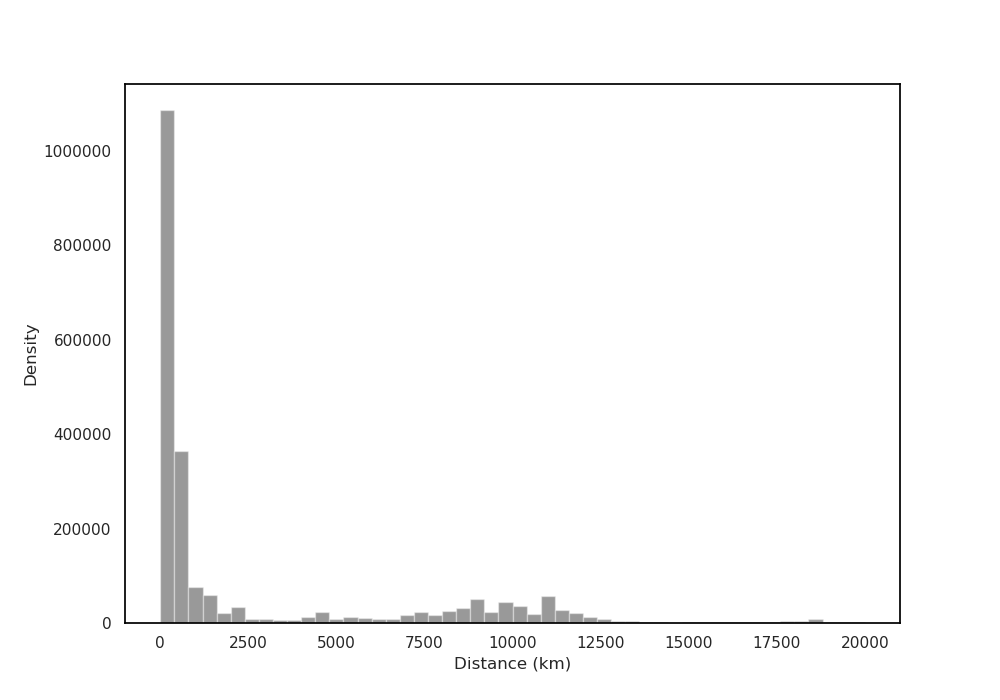
\includegraphics[width=1\textwidth]{images/distance_frequency.png}
    
    \caption{Distribution of Distances}
    \label{fig:distribution-distances}
\end{figure}

Figure \ref{fig:distribution-distances} shows distribution of all distances (not taking into account that some tweets have duplicate locations).

\begin{figure}[H]
    \centering
    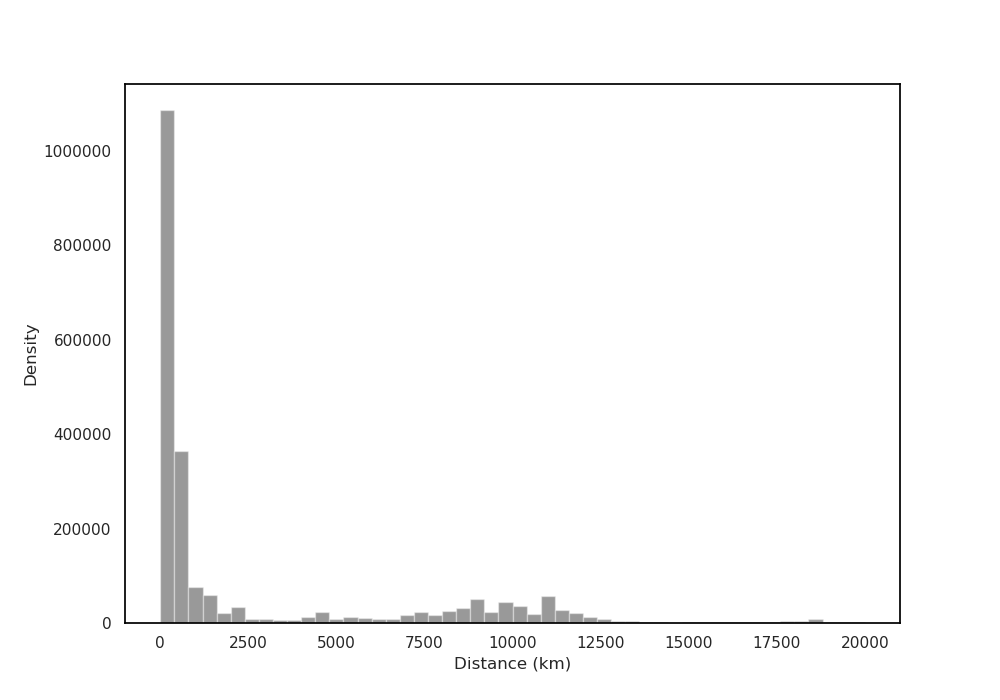
\includegraphics[width=1\textwidth]{images/distance_frequency.png}
    
    \caption{Distribution of Distances}
    \label{fig:distance-frequency}
\end{figure}

482,741 of tweets had a geoparsed country and a geotagged country that was the same, and in 868,020 tweets the geoparsed and geotagged tweets were different (considering duplicates due to multiple geoparsed toponyms per tweet).

\subsection{If Argentina was mentioned, where were the geotags?}

444333 of the geotags in this subset of the data corresponded to Argentina, corresponding to over 96\%. So Argentina was filtered out to get a better understanding of geotagged countries.

\begin{table}[H]
\centering
\begin{tabular}{lcc}
\hline
Country & Counts & Proportion \\
\hline
Brazil & 2454 & 0.136409 \\
USA & 2344 & 0.130295 \\
Chile & 1476 & 0.082046 \\
Uruguay & 874 & 0.048583 \\
Mexico & 682 & 0.037910 \\
Spain & 623 & 0.034630 \\
Peru & 456 & 0.025347 \\
Paraguay & 445 & 0.024736 \\
Italy & 363 & 0.020178 \\
France & 337 & 0.018733 \\
Colombia & 335 & 0.018621 \\
United Kingdom & 315 & 0.017510 \\
Ecuador & 262 & 0.014564 \\
Dominican Republic & 221 & 0.012285 \\
Japan & 220 & 0.012229 \\
Bolivia & 209 & 0.011618 \\
Canada & 195 & 0.010839 \\
Germany & 171 & 0.009505 \\
Indonesia & 165 & 0.009172 \\
Other & 5679 & 0.315675 \\
\hline
\end{tabular}
\caption{Country Counts and Proportions}
\label{tab:distances-argentina-mentioned}
\end{table}


\subsection{If the geotag is Argentina, what are the mentions?}

Again, Argentina was filtered out for the same reason as above.

\begin{table}[H]
\centering
\begin{tabular}{lcc}
\hline
Country & Counts & Prop \\
\hline
USA & 126,511 & 0.267 \\
Brazil & 28,233 & 0.060 \\
Italy & 27,680 & 0.058 \\
Spain & 25,060 & 0.053 \\
Chile & 20,070 & 0.042 \\
Mexico & 18,613 & 0.039 \\
France & 16,267 & 0.034 \\
United States & 11,555 & 0.024 \\
Colombia & 11,449 & 0.024 \\
Uruguay & 8,679 & 0.018 \\
Venezuela & 8,553 & 0.018 \\
UK & 7,694 & 0.016 \\
Puerto Rico & 7,634 & 0.016 \\
Peru & 5,891 & 0.012 \\
Bulgaria & 5,789 & 0.012 \\
China & 5,726 & 0.012 \\
Japan & 5,562 & 0.012 \\
Paraguay & 5,325 & 0.011 \\
Germany & 5,126 & 0.011 \\
Other & 116,800 & 0.247 \\
\hline
\end{tabular}
\caption{Argentina Geotagged}
\label{distances-argentina-geotagged}
\end{table}

The top 30 geotagged countries and top 30 geoparsed countries were found, and their intersection was found. For the resulting 20 countries, a heatmap was produced. 

\begin{figure}[H]
    \centering
    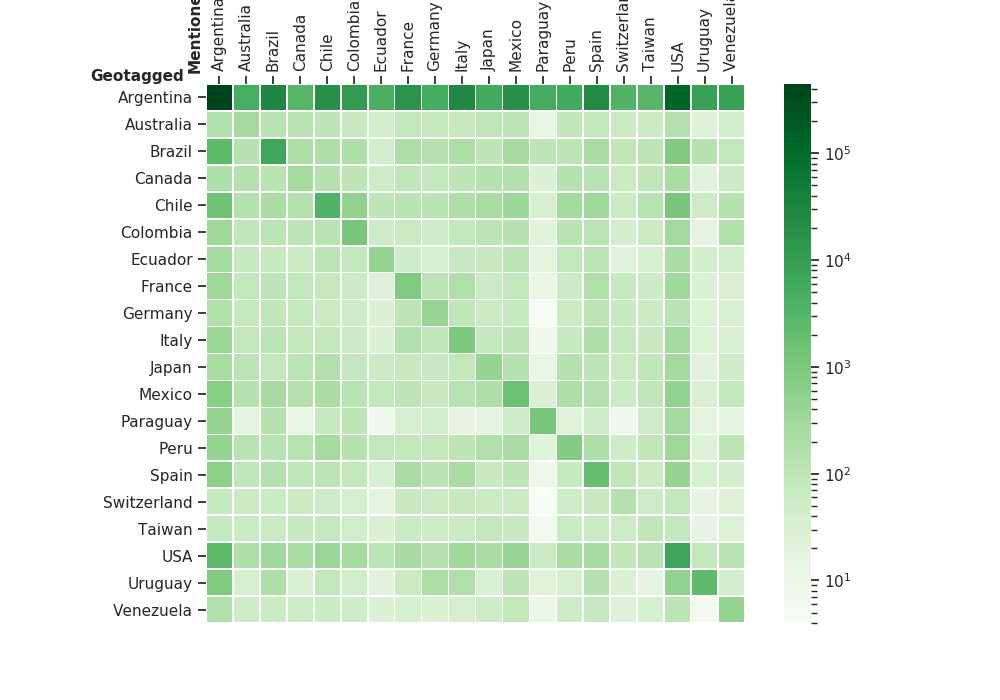
\includegraphics[width=1\textwidth]{images/distance-heatmap.png}
    
    \caption{Number of Tweets With Geotagged Country vs Mentioned (Geoparsed) Country Heatmap}
    \label{fig:distance-heatmap}
\end{figure}
